\documentclass[../../main.tex]{subfiles}
\begin{document}


\subsection{Control System Design Based on Model}
% introduction, quickly describe which tunings methods are to be explored. List the specifications which are attempted to be met.
%If it is not already mentioned earlier, mention that the design is done by assuming the controller to be continuous rather than discretising the plant
As mentioned in section \ref{} the controller design method explored in this project will focus on different configurations of a PID controller. Both single and cascaded controllers will be examined, meaning that both position and velocity controllers is to be designed. The main focus will be on comparing different controller configurations more than achieving a specified performance. Tough a performance specification has been listed, in order for easier comparing of methods. The performance specifications can be seen in table \ref{tab:performanceSpec}.

As mentioned in section \ref{sec:Delimination} the controllers designed in this section will be designed in the continuous time domain, afterwards additional steps will be taken to approximate the effect of the discrete controller, and verify performance.

\begin{table}[]
    \centering
    \begin{tabular}{lc}
        Rise time &  0.5 \si{\sec}\\
        Settling time & 1.5 \si{\sec}\\ 
        Overshoot & 5 \%
    \end{tabular}
    \caption{Performance specifications}
    \label{tab:performanceSpec}
\end{table}



% Position 
% Present the bode plot of closed loop and argue that the chosen sampling rate is sufficient.
% Inserting a delay to emulate the discrete controller, present the stability margins
% Argue why the specific reference is used for the step response
% block diagram representing the controller with, and without saturation. Showing step responses with and without saturation, argue that for future responses, a model with saturation is used, in order be able to compare to tests. Maybe also present an argument for anti wind-up, if not presented previously.
%looking at the step response, discuss how well it matches the specifications
A relatively simple control system is to design a single PID controller for the position, which controls the voltage supplied to the pan and tilt motors based on a position feedback. Such a controller should be designed for both the pan and the tilt motor. To aid the design of the control systems, meaning calculating the correct gains for the proportional, integral and derivative terms, the Root Locus plot will be utilised. Considering a closed loop system of the form shown in equation \ref{eq:closedLoopSystem}, with a proportional controller $K$ and plant $G(s)$, the Root Locus shows how the closed loop poles move as the gain of the controller changes. With a high enough gain, the closed loop poles will move either towards the open loop zeros or infinity. By designing a controller to strategically place zeros, and choosing an appropriate gain, the position of the closed loop poles can be controlled.
\begin{equation}\label{eq:closedLoopSystem}
    \frac{K\cdot G(s)}{1+K\cdot G(s)}
\end{equation}
As seen from the transfer function of a PID controller in equation \ref{eq:PID_transfer_function},where $k_p$,$k_d$ and $k_i$ are the gains, this type of controller adds two open loop zeros and one open loop pole to an existing system. The open loop pole, originating from the integral term, will always be placed at the origin, but the zero positions can be controlled.
\begin{equation}\label{eq:PID_transfer_function}
    K(s) = \frac{K_d s^2 + K_p s + K_i}{s}
\end{equation}

The design procedure which will be followed in this section will thus involve first placing these two zeros and afterwards choosing an appropriate gain based on the Root Locus plot. To place the zeros, equation \ref{eq:PID_zero_placement} is used, where $-z_1$ and $-z_2$ describe zero positions.
\begin{equation}\label{eq:PID_zero_placement}
    K(s) = \frac{(s+z_1)\cdot(s+z_2)}{s}
\end{equation}
To figure out where to place the zeros, it must first be considered where the poles for the closed loop system should ideally be placed. In order to achieve the predominant goal of having a stable system, all closed loop poles must first of all be placed to the left of the imaginary axis in the complex plane. To further determine appropriate locations for the poles, one must consider the time domain specifications, shown in table \ref{tab:performanceSpec}, which have been set up for the system. These can be used produce some frequency domain rules which indicate an area in the complex plane in which the poles should be located to honour the specifications. These rules are based on the transfer function in equation \ref{eq:basic_second_order_tf}, which is a second order system without zeros. The closed loop system for position control has four poles, although only three dominant ones, and two zeros, so these rules will be used as guidelines. To obtain a rise time shorther than $t_r$ the minimum magnitude, $w_n$, of the poles can be approximated as $w_n\geq\frac{1.8}{t_r}$. To obtain a 1\% settling time faster than $t_s$, the magnitude of the real part of the poles, $\sigma = \omega_n \zeta$ can be found as $\sigma \geq \frac{-\ln{0.01}}{t_s} $. Lastly, to keep an overshoot below 5\%, it must be true that $\zeta \geq \sqrt{\frac{(\frac{\ln{0.05}}{-\pi})^2}{1+(\frac{\ln{0.05}}{-\pi})^2}}$, which defines a cone shaped region in the complex plane, in which the poles should be placed. The lines indicating the region based on the specifications can be seen on the figure \ref{fig:system_requirements}.
% remember that the poles have to be in the left half plane, introduce how the specifications map to the root locus plot.
\begin{equation} \label{eq:basic_second_order_tf}
    H(s) = \frac{\omega_n^2}{s^2 + 2\zeta \omega_n s + \omega_n^2}
\end{equation}
\begin{figure}
    \centering
    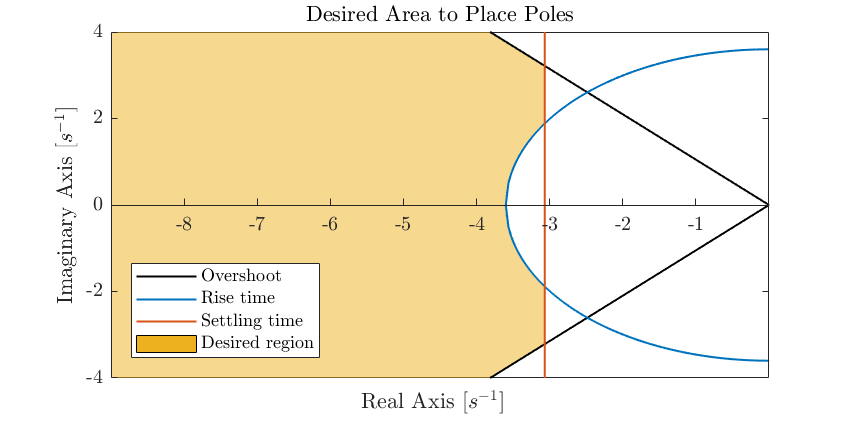
\includegraphics[width=0.7\textwidth]{Sections/System_Design/Images/system_requirements_new.png}
    \caption{All poles should be placed to the left of all the lines, in the yellow region, for the system to meet the required performance}
    \label{fig:system_requirements}
\end{figure}

It can be seen on figure \ref{fig:PosRootLocus} that in order to follow the frequency domain guidelines found above, the two open loop poles at the origin should be moved to the left, while at the same time keeping their imaginary parts close enough to zero to stay within the cone shaped region dictated by the requirement of 5\% overshoot.
Through experimentation it has been found that placing zeros at $9.5$ and $1$ for the tilt motor and at $3.3$ and $0.8$ for the pan motor, produced satisfactory Root Loci, which are shown in figure \ref{fig:PosRootLocus}. Based on the plots, an appropriate gain is chosen. For the tilt motor a value of $0.9$ was chosen while $1.2$ was chosen for the pan motor. This results in the control gains shown in table \ref{tab:pos_controller_gains}. The closed loop pole locations at these gains are also visible from figure \ref{fig:PosRootLocus}.


\begin{figure}[h]
\begin{subfigure}{0.48\textwidth}
    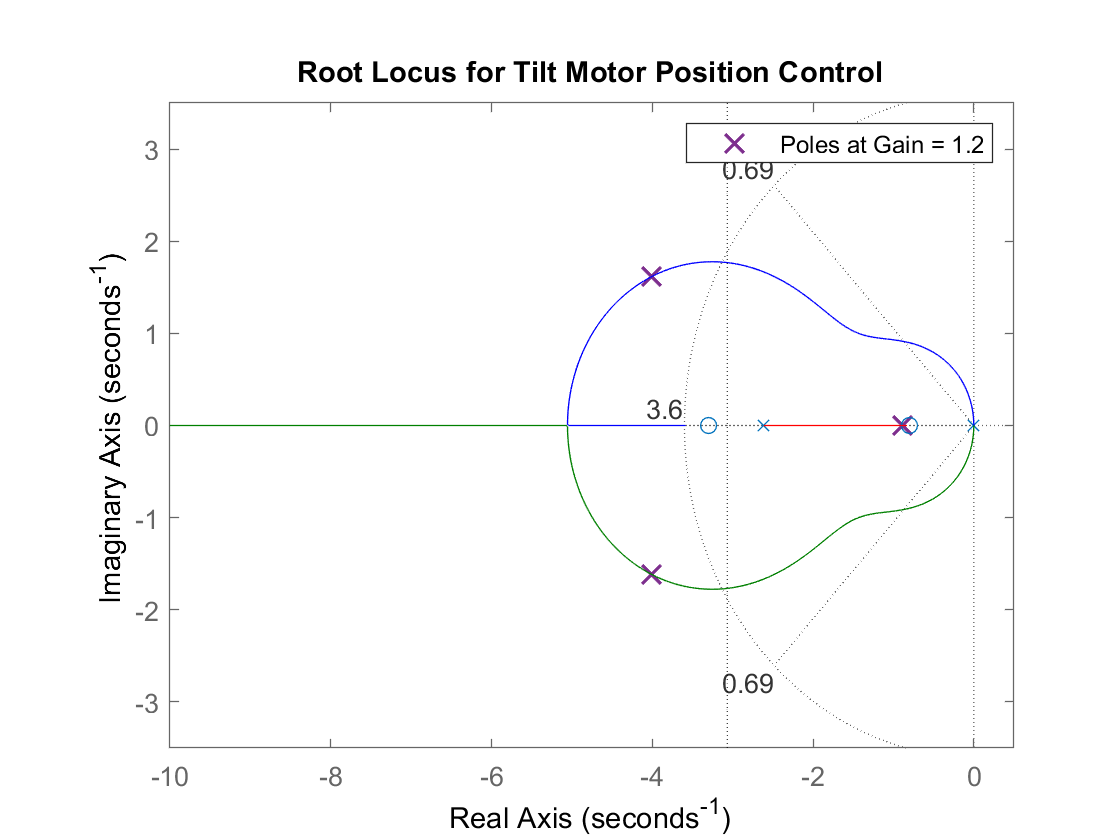
\includegraphics[width = 0.97\textwidth]{Sections/System_Design/Images/RL_PanMotorPos2.png}
    \caption{Root locus pan motor}
    \label{fig:PosRootLocusPan}
\end{subfigure}\quad
\begin{subfigure}{0.48\textwidth}
    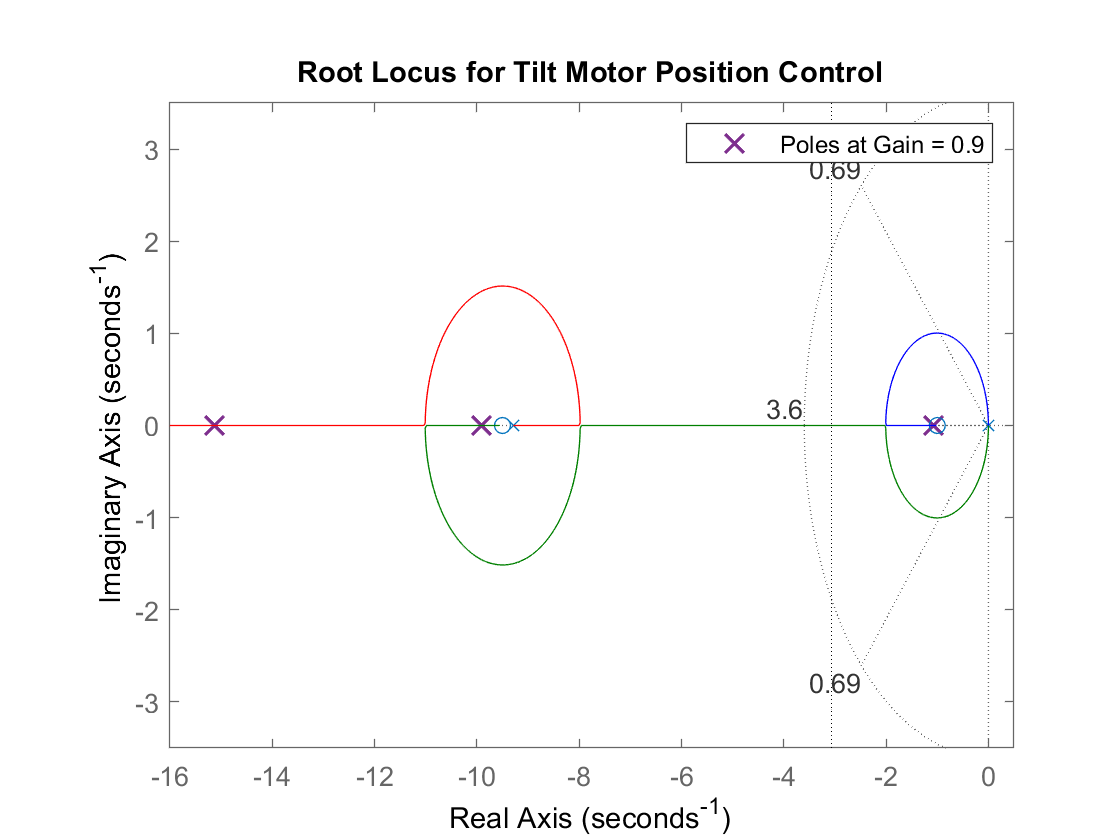
\includegraphics[width = 0.97\textwidth]{Sections/System_Design/Images/RL_TiltMotorPos.png}
    \caption{Root locus tilt motor}
    \label{fig:PosRootLocusTilt}
\end{subfigure}
\caption{}
\label{fig:PosRootLocus}
\end{figure}

\begin{figure}[h]
    \centering
    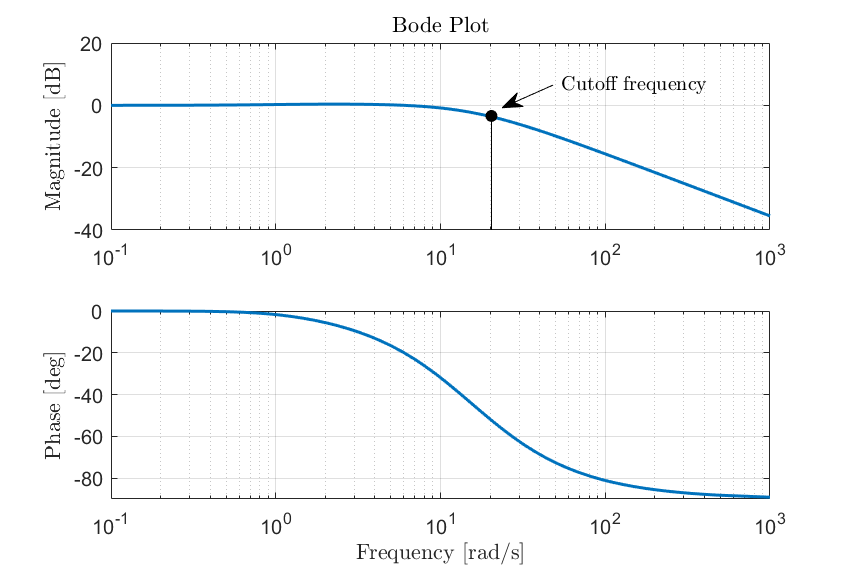
\includegraphics[width=0.65\textwidth]{Sections/System_Design/Images/Bode_TiltMotorPos.png}
    \caption{Bode plot of the closed loop control system for the tilt motor.}
    \label{fig:pos_bode_plot}
\end{figure}

A rule of thumb states that when implementing a continuously designed controller in a discrete system, such as a micro controller, the sampling frequency shall be 25-30 times the bandwidth of the closed loop system. A bode plot of the closed loop system for the tilt motor, shown in figure \ref{fig:pos_bode_plot} reveals a cut off frequency of \SI{18}{\radian \per \second}. The tilt motor bode plot is highlighted since it has the highest bandwidth. A similar plot for the pan motor can be found in the digital appendix, where future bode plots referenced in this section can also be found, which is outlined in section \ref{sec:digital_appendix}. It has been decided to implement the position controllers using a sampling frequency of \SI{1000}{\hertz}. This easily honours the the rule of thumb, which would demand a sampling time of $t_{sampling} = \frac{18}{2\pi}\cdot 30 = \SI{85.94}{\hertz}$.
To emulate the discrete controller, a delay of half of the sampling time is added to the controller. This is done by adding the the transfer function shown in equation \ref{eq:delay_transfer_function}, with $t_{sampling} = \SI{0.001}{\second}$, to the transfer function of the PID controller. 
\begin{equation}\label{eq:delay_transfer_function}
    G_{delay}(s) = \frac{1}{\frac{t_{sampling}}{2}\cdot s+1}
\end{equation}
With this delay added, the phase and gain margins are evaluated by drawing the bode plot of the open loop transfer function and evaluating the phase at the frequency which gives  \SI{0}{\deci \bel} gain, and evaluating the gain at the frequency which gives \SI{-180}{\degree} phase. As seen in figure \ref{fig:pos_stability_plot}, the gain margins for the tilt and pan motors are \SI{100}{\deci \bel} and \SI{105}{\deci \bel} respectively, while the phase margins are \SI{85.6}{\degree} and \SI{77.9}{\degree}. These margins are quite large, which is good, since that allows room for more uncertainties in the plant model.

\begin{figure}[h]
\begin{subfigure}{0.48\textwidth}
    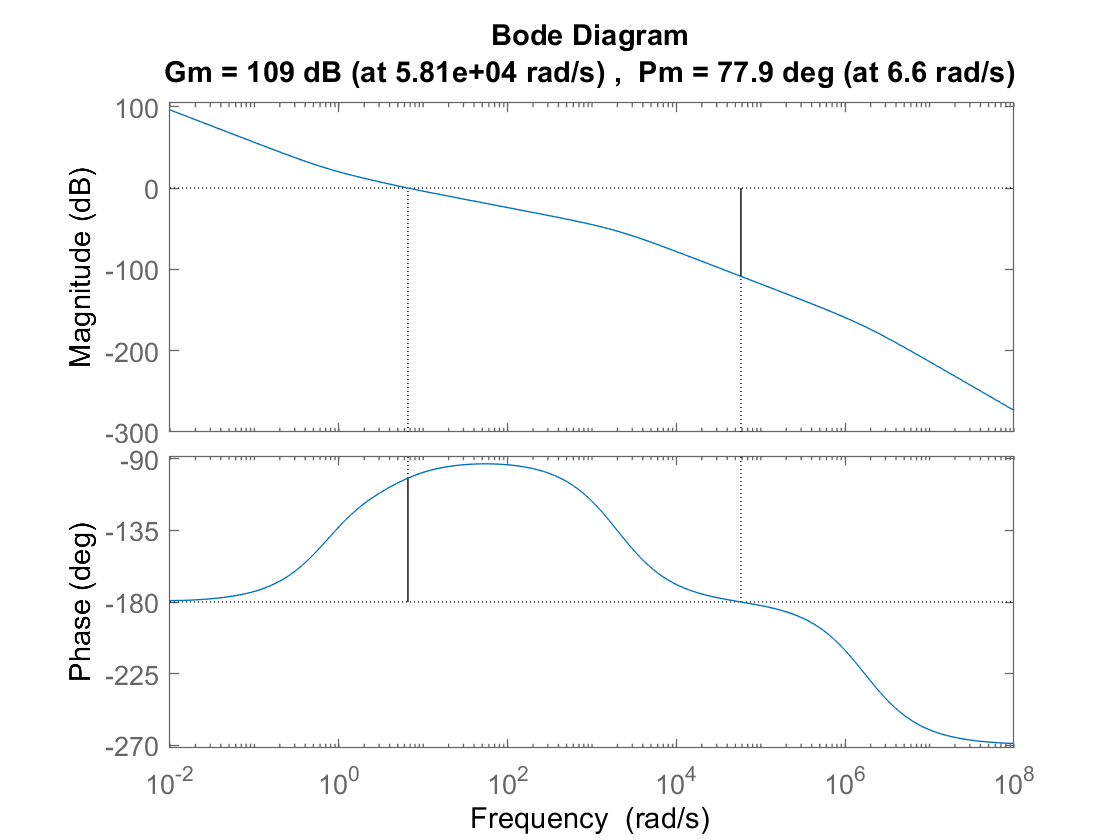
\includegraphics[width = 0.97\textwidth]{Sections/System_Design/Images/SM_PanMotorPos2.png}
    \caption{Pan motor.}
    \label{fig:pos_stability_plot_pan}
\end{subfigure}\quad
\begin{subfigure}{0.48\textwidth}
    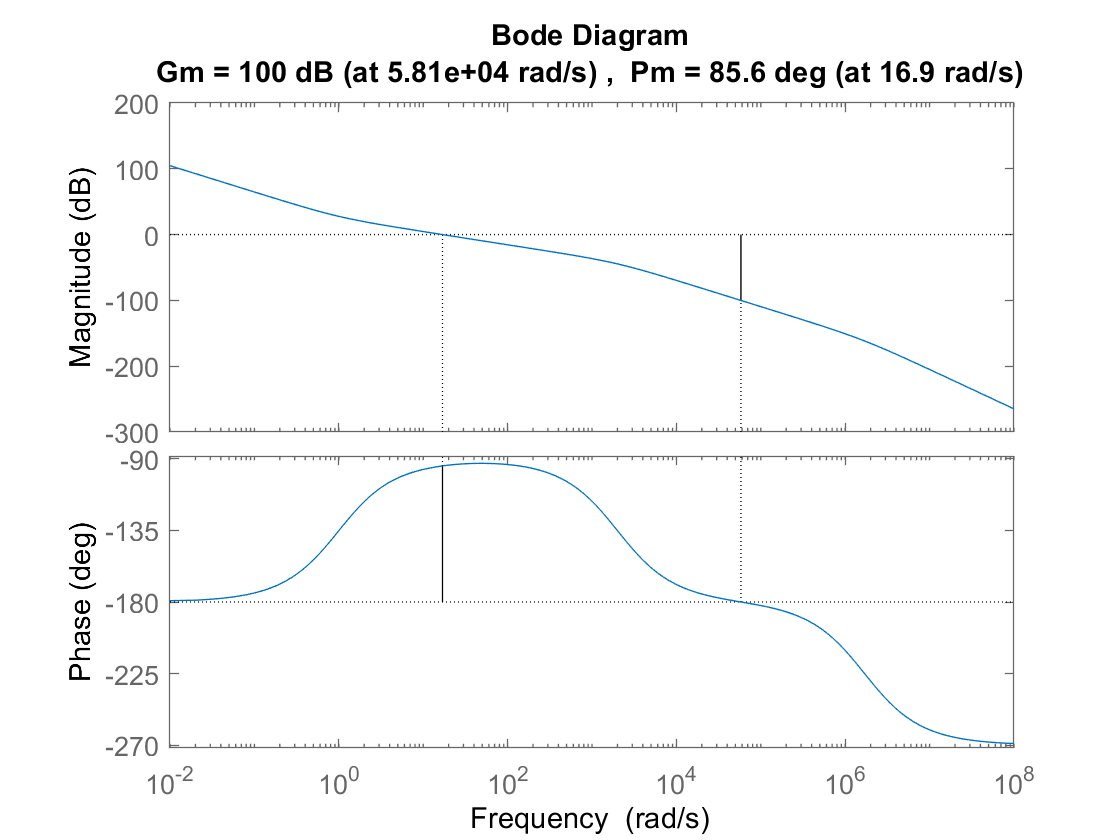
\includegraphics[width = 0.97\textwidth]{Sections/System_Design/Images/SM_TiltMotorPos.png}
    \caption{Tilt motor.}
    \label{fig:pos_stability_plot_tilt}
\end{subfigure}
\caption{Bode plots of the closed loop motor control systems for the pan and tilt motors.}
\label{fig:pos_stability_plot}
\end{figure}

To verify the performance of the controllers, the tilt and pan motor systems, with added PID controllers, are simulated using a step reference of magnitude 1. To properly emulate the physical system, saturation and associated anti wind-up must be added as seen on figure \ref{}, since the physical system can only respond to a limited control signal. Figure \ref{fig:PosStepSat} and \ref{fig:PosStepNoSat} show the difference that the saturation makes. It shows that ideally, the controller for the tilt motor honours the specifications, however the specifications for settling time and overshoot are not quite met when saturation is introduced. Also, even without the saturation, the step response of the pan motor controller does not quite live up to the  requirements, but through experimenting with different zero placement and gains, it was found to be the best compromise between a relatively fast rise and settling time, while still keeping the overshoot reasonable.

\begin{figure}[h]
\begin{subfigure}{0.48\textwidth}
    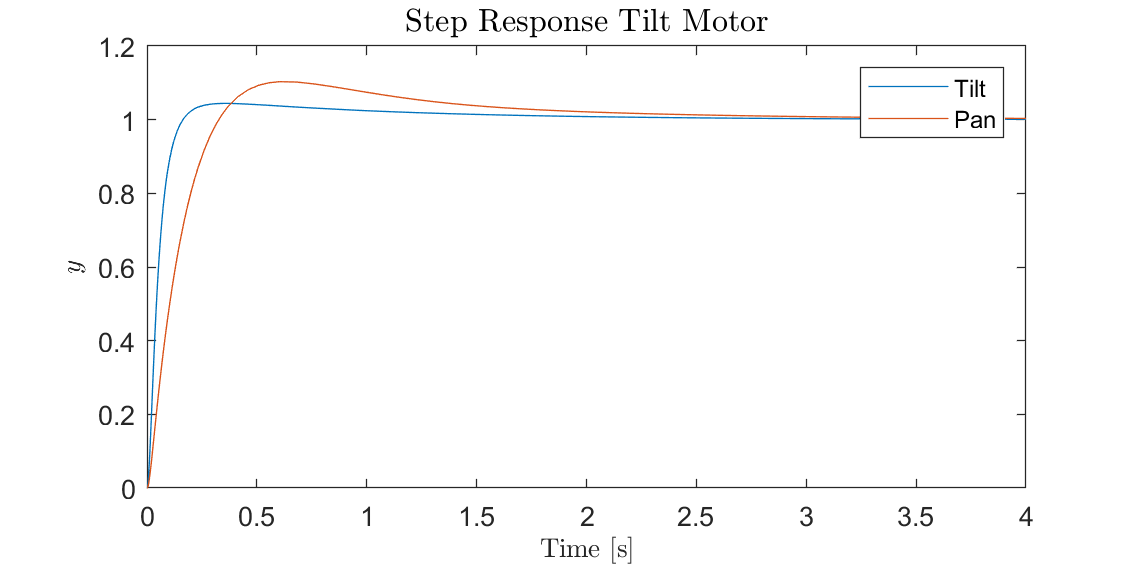
\includegraphics[width = 0.97\textwidth]{Sections/System_Design/Images/Pos_step_y_1_noSat.png}
     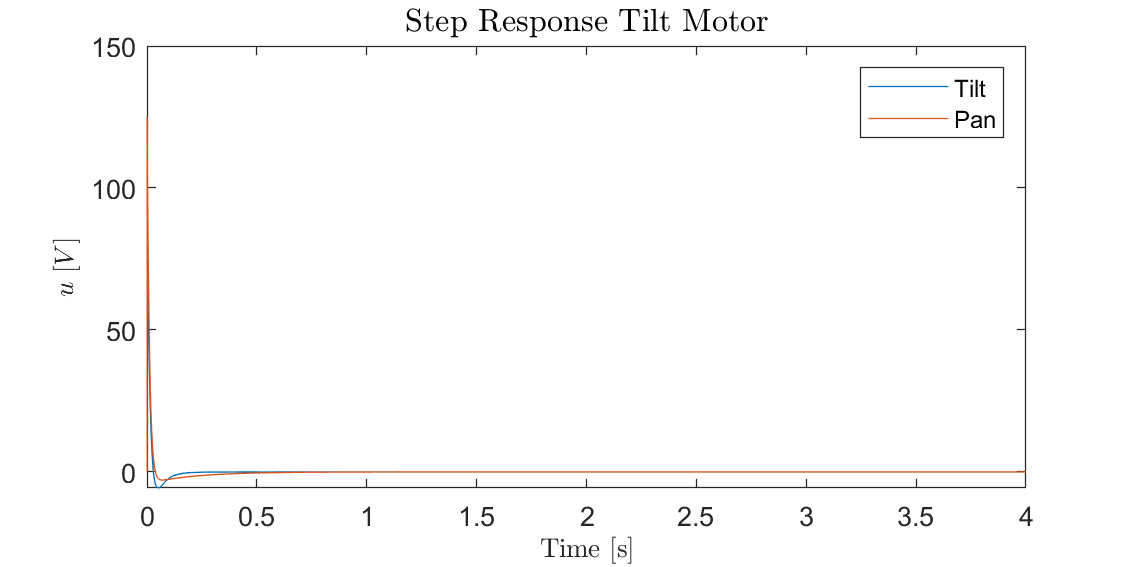
\includegraphics[width = 0.97\textwidth]{Sections/System_Design/Images/Pos_step_u_1_noSat.png}
    \caption{Without saturation.}
    \label{fig:PosStepSat}
\end{subfigure}\quad
\begin{subfigure}{0.48\textwidth}
    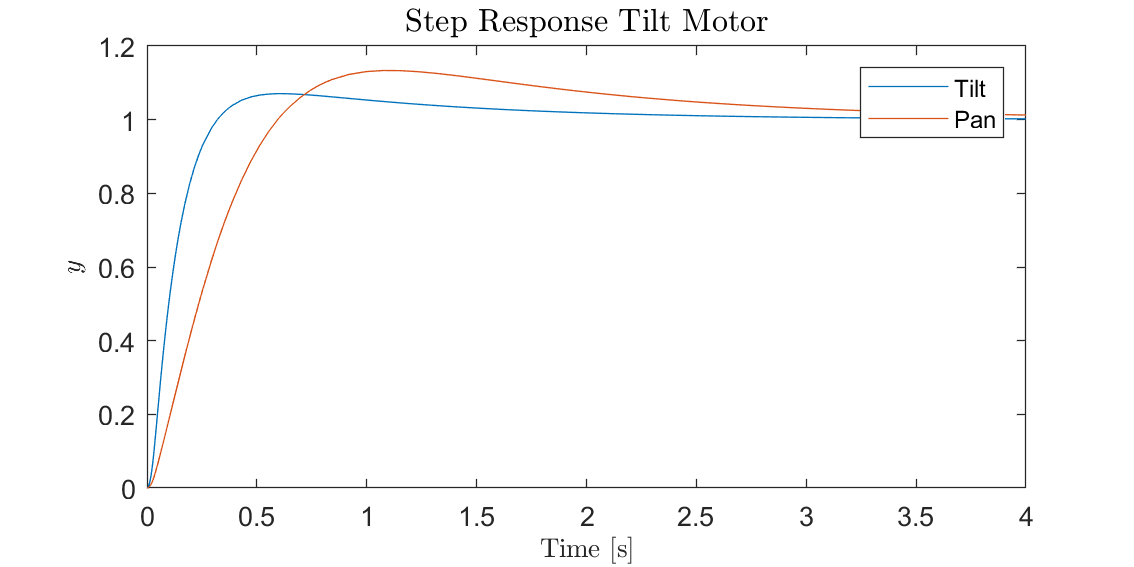
\includegraphics[width = 0.97\textwidth]{Sections/System_Design/Images/Pos_step_y_1_Sat.png}
    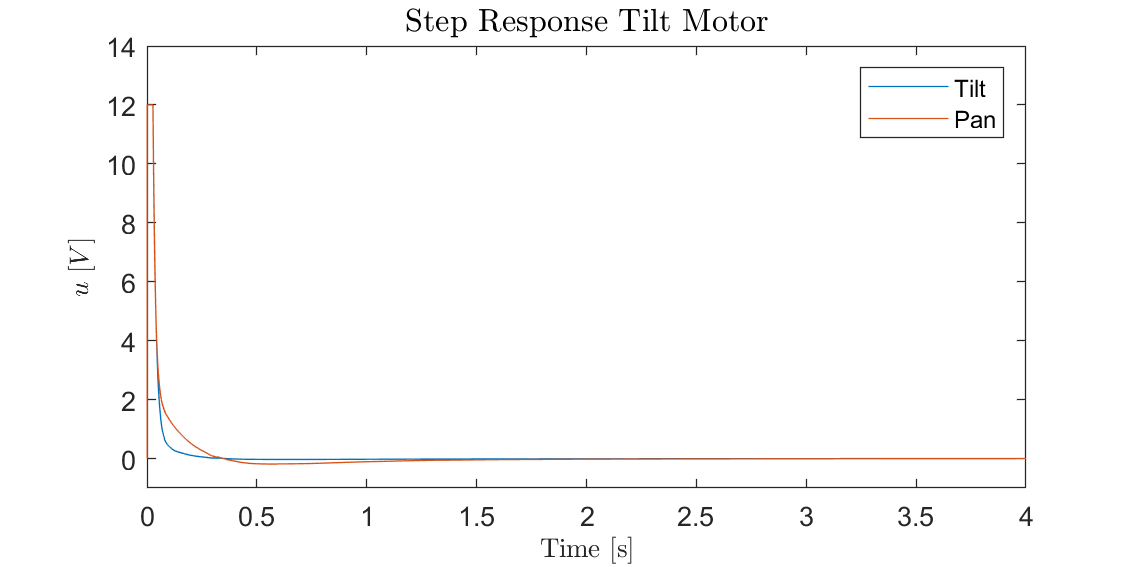
\includegraphics[width = 0.97\textwidth]{Sections/System_Design/Images/Pos_step_u_1_Sat.png}
    \caption{With saturation.}
    \label{fig:PosStepNoSat}
\end{subfigure}
\caption{Step responses of the designed control systems with and without saturation taken into account.}
\label{fig:PosStep}
\end{figure}


\subsection{Velocity Controller Design}
As mentioned in section \ref{sec:Delimination}, it is wanted to explore the performance of a cascaded controller design. To achieve this, a velocity controller must be designed. The range of motion for the pan motor is physically fairly limited. Therefore it has been prioritized to focus on designing a velocity controller for the tilt motor, as the unlimited range makes testing the velocity controller, without jeopardising the pan/tilt system, easier. Two different methods of designing velocity controllers will be explored. One will use the pole placement approach used above, the other will utilize the Ziegler-Nichols approach, which can be used without a mathematical model of the system to be controlled.

\subsubsection{Ziegler-Nichols Tuning}
%The Ziegler-Nichols tuning method provides a method for tuning a PID controller without knowing specific information about the dynamics of the plant. 
Instead of analysing a mathematical model of the plant, the Ziegler-Nichols method uses the step response of the physical system to calculate the controller gains. when using the Ziegler-Nichols method it is not possible to dictate performance specification. Instead, the obtained closed-loop system always will have a decay ratio, $\zeta$, of approximately 0.25. The method assumes that the plant can be described by a delayed first order system of the form seen in equation \ref{eq:NZ_plant_eq}

\begin{equation}
    \frac{y(s)}{u(s)} = \frac{A}{\tau s + 1} e^{-s t_d}
    \label{eq:NZ_plant_eq}
\end{equation}

To calculate the controller gains a set of equations are provided. The equations differ depending on the controller type, the equations used for calculating the gains for a PID controller can be seen in equations \ref{eq:controllerGains}. The constants R and L are identified from the step response. The constant R is found by drawing the tangent to the steepest part of the transition between zero and the reference. The gradient of the tangent is equal to R. L is equal to the latency of the system, and is defined as the distance between the y-axis and the intersection between the tangent and the x-axis. 

\begin{equation}
k_p = \frac{1.2}{RL}, \quad k_i = \frac{k_p}{2L}, \quad k_d = \frac{k_p}{0.5L}
\label{eq:controllerGains}
\end{equation}

The Ziegler-Nichols tuning method has only been used to tune the velocity controller due to only being possible to obtain a velocity step response. Furthermore it has not been possible to get the velocity from the pan motor due to limitations on the rotation of the frame. Therefore the Ziegler-Nichols has only been used to tune the velocity controller for the tilt motor.

\begin{figure}
    \centering
    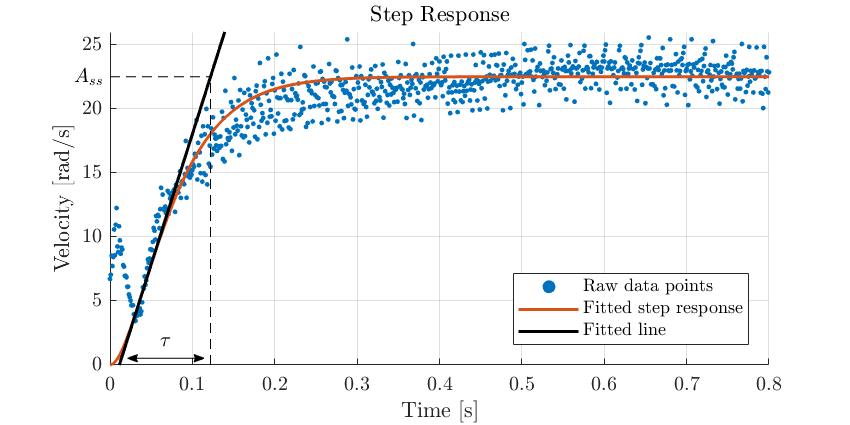
\includegraphics[width = 1\textwidth]{Sections/System_Design/Images/Ziegler-Nichols_Stepresponse.png}
    \caption{Velocity step response for the actual tilt motor, used for tuning using Ziegler-Nichols.}
    \label{fig:stepPlantNZ}
\end{figure}

In figure \ref{fig:stepPlantNZ} the data point sampled from the step response of the physically  system is plotted. The Curve Fitting tool in MATLAB has then been used to fit a curve that fits the points, it is displayed as the red line. The red line is described as the expression introduced in equation \ref{eq:NZ_plant_eq}.
From the fitted line the tangent is then found. From the MATLAB console R and L read as seen in equation \ref{eq:R_and_L}.

\begin{equation}
    R = 203.4 \quad L = 11.4 \cdot 10^{-3} 
    \label{eq:R_and_L}
\end{equation}

Using the found values for R and L from equation \ref{eq:R_and_L} and the equations introduced in equation \ref{eq:controllerGains} the controller gains found as seen in equation \ref{eq:controllerGainsCal}

\begin{equation}
    k_p = 0.5194, \quad k_i = 22.86, \quad k_d = 3.0 \cdot 10^{-3}
    \label{eq:controllerGainsCal}
\end{equation}


\begin{figure}
    \centering
    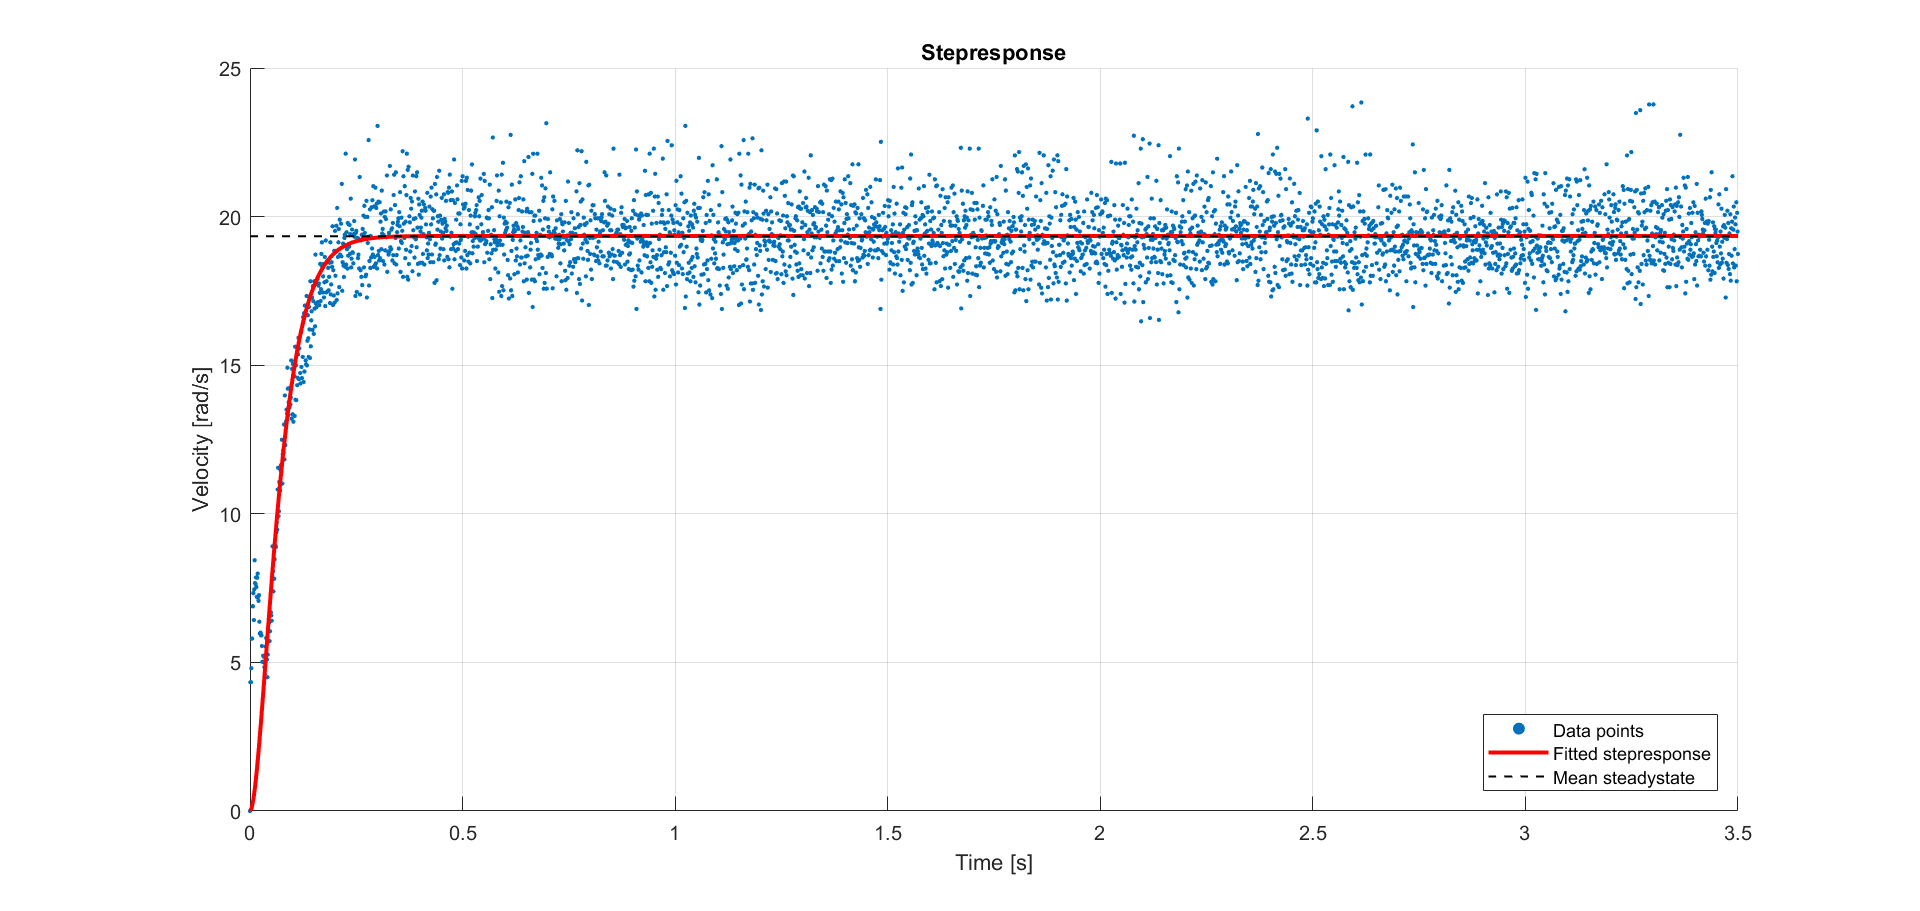
\includegraphics[width = 1\textwidth]{Sections/System_Design/Images/Step_Implemented_NZ.png}
    \caption{Closed-loop velocity step response of the controller tuned using Ziegler-Nichols.}
    \label{fig:NZ_implemented}
\end{figure}


In figure \ref{fig:NZ_implemented} the measured step response using the calculated gains seen in equation \ref{eq:controllerGainsCal} is plotted. 

(Kom med forklaring på, hvorfor der er steady state error)

\subsubsection{Model Based Controller Design}
When working with a cascaded control design, it is desired that any inner controllers are faster than the outer loop, as well as critically or over damped. It is therefore worked towards designing a controller yielding no overshoot while still achieving a fast rise time.
The procedure for designing the velocity controller based on the model is very similar to the approach used for designing the position controllers above. The main difference is that open loop system now has one less pole at the origin, as the only pole at the origin originates from the integral term of the PID controller. As seen on figure \ref{fig:vel_root_locus}, it has been found that placing the zeros accruing to the PID controller at $s = -10$ and $s = -12$, yields adequate Root Loci. This placement allows the close loop poles to be moved fairly far into the left half plane, while still remaining directly on the real axis. A gain value of $0.065$ is chosen. The closed loop pole locations are also visible from the figure. The closed loop pole and zero locations can be compared to the pole and zero locations given by the Ziegler-Nichols tuning shown in figure \ref{fig:ZN_pole_zero}.

\begin{figure}[h]
\begin{subfigure}{0.48\textwidth}
    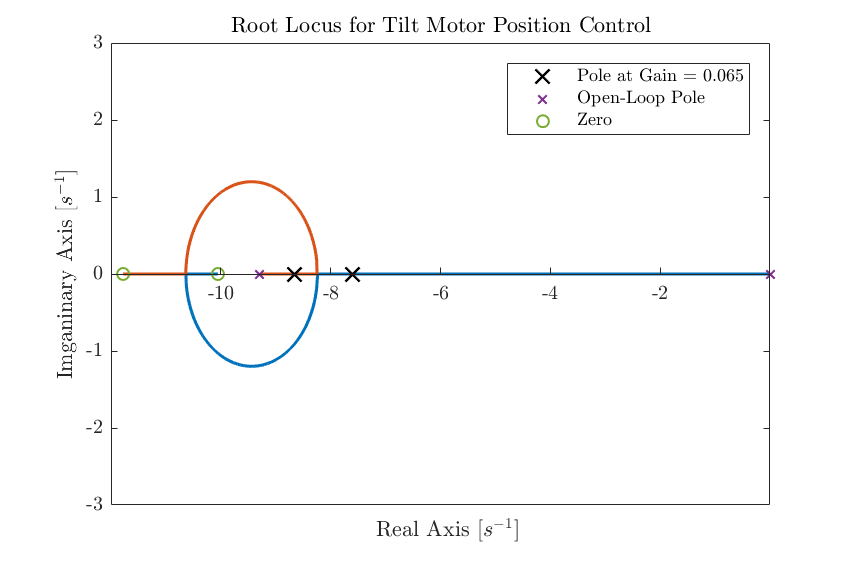
\includegraphics[width = 0.97\textwidth]{Sections/System_Design/Images/RL_TiltMotorVelPolePlace.png}
    \caption{Pan motor.}
    \label{fig:vel_root_locus}
\end{subfigure}\quad
\begin{subfigure}{0.48\textwidth}
    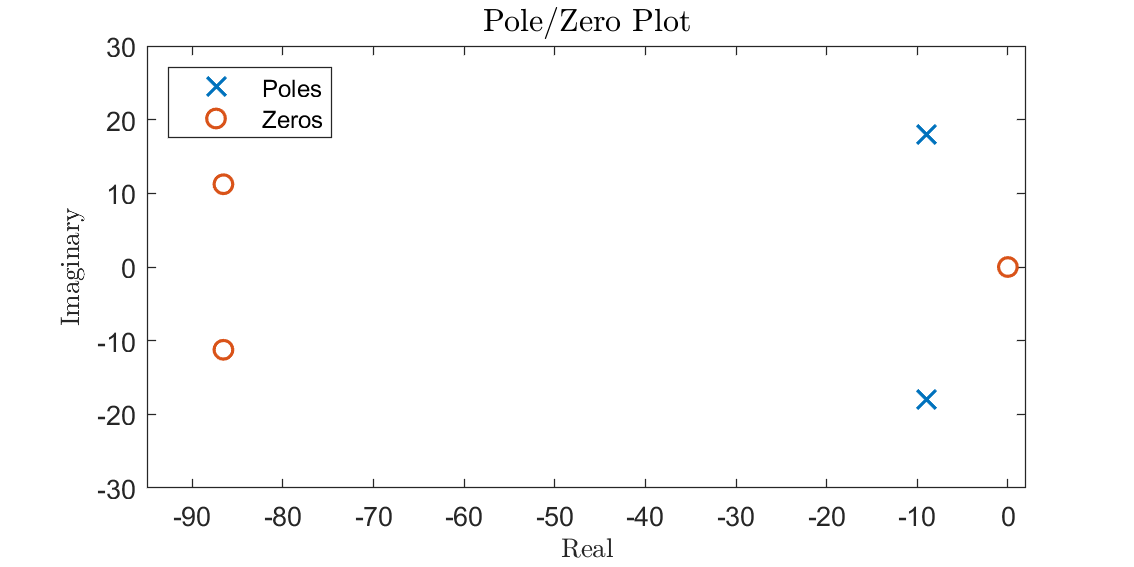
\includegraphics[width = 0.97\textwidth]{Sections/System_Design/Images/PoleZero_TiltMotorVel_NZ.png}
    \caption{Closed loop poles and zero locations obtained via using the Ziegler-Nichols tuning method.}
    \label{fig:ZN_pole_zero}
\end{subfigure}
\caption{Bode plots of the closed loop motor control systems for the pan and tilt motors.}
\label{fig:vel_poles_zeros}
\end{figure}

As with the position controller, the bandwidth of the closed loop velocity controller systems are evaluated. The cut off frequencies are found to be at just about \SI{11}{\radian \per \second} for the model based design, and just about \SI{28}{\radian \per \second} for the Ziegler-Nichols based design. Therefore it can be concluded that the chosen sampling frequency of \SI{1000}{\hertz} is again more than sufficient. It is worth mentioning however, that a higher band width would have been preferable, especially for the model based controller. 
The phase and gain margins are also examined for the velocity controller, again with the delay introduced to emulate the discrete controller. 
From figure \ref{fig:vel_stability_plot} it can be seen that both design approaches gives an infinite gain margin, as the phase never crosses \SI{-180}{\degree}. It is worth noting however, that the Ziegler-Nichols based design has significantly less phase margin. The \SI{50}{\degree} phase margin is still deemed sufficient though.
% As seen in figure \ref{fig:vel_stability_plot}, large stability margins are obtained. The gain margin is infinite as the phase never crosses \SI{-180}{\degree} and the phase margin is found to be \SI{145}{\degree}. It is worth mentioning though, that the magnitude plot does show a flat band just around a gain of \SI{0}{\deci \bel}. This means that the phase margin could be quite different given just a slight change in gain. Looking at the figure however, it can be seen that the phase margin would still remain about the same, or even increase.
% comment on the bode plot and stability
% comment on the step response that the goal are reached.

% \begin{figure}[h]
% \begin{subfigure}{0.48\textwidth}
%     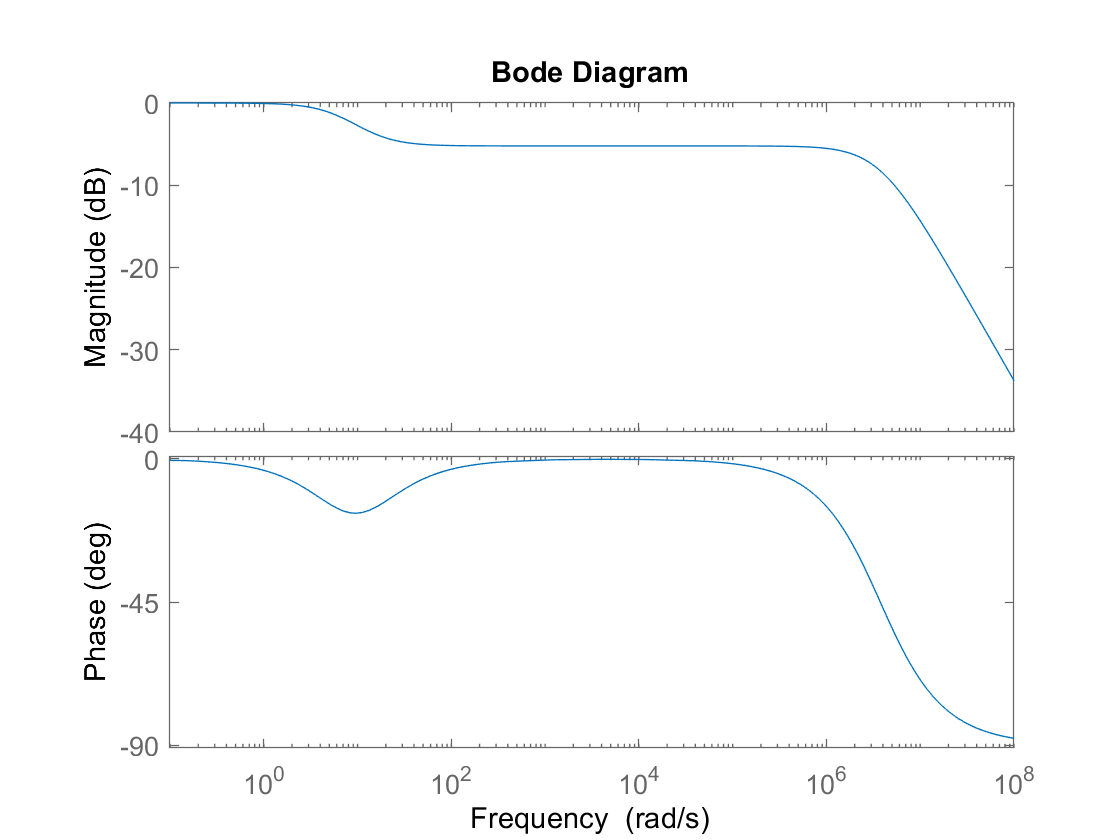
\includegraphics[width = 0.97\textwidth]{Sections/System_Design/Images/Bode_TiltMotorVel_polePlace.png}
%     \caption{Controller design based on model}
%     \label{fig:vel_PP_bode_plot}
% \end{subfigure}\quad
% \begin{subfigure}{0.48\textwidth}
%     \includegraphics[width = 0.97\textwidth]{}
%     \caption{Maybe add the bode plot the ziegler nichols here.}
%     \label{fig:vel_ZN_bode_plot}
% \end{subfigure}
% \caption{Bode plots of the closed loop system with velocity controllers designed using the model and using the Ziegler-Nichols method.}
% \label{fig:vel_bode_plots}
% \end{figure}

\begin{figure}[h]
\begin{subfigure}{0.48\textwidth}
    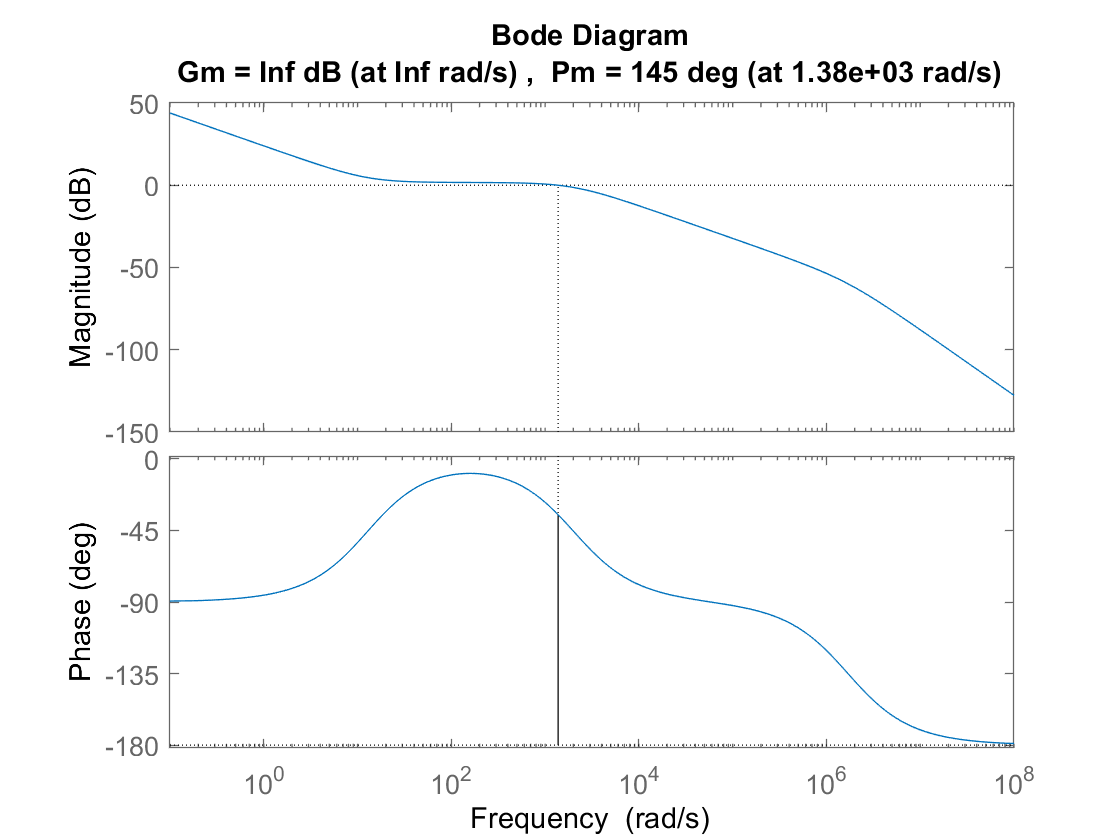
\includegraphics[width = 0.97\textwidth]{Sections/System_Design/Images/SM_TiltMotorVel_polePlace.png}
    \caption{Controller design based on model.}
    \label{fig:vel_PP_stability_plot}
\end{subfigure}\quad
\begin{subfigure}{0.48\textwidth}
    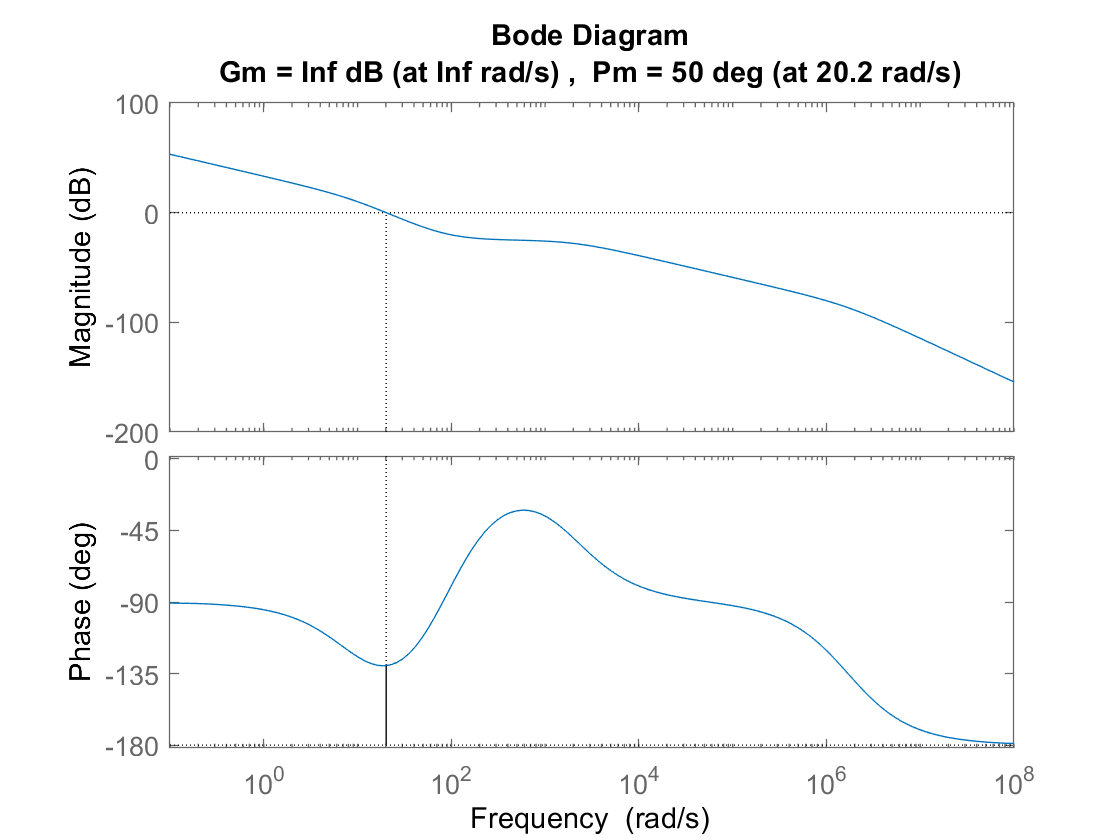
\includegraphics[width = 0.97\textwidth]{Sections/System_Design/Images/SM_TiltMotorVel_NZ.png}
    \caption{Controller design based on Ziegler-Nichols.}
    \label{fig:vel_ZN_stabilty_plot}
\end{subfigure}
\caption{Bode plots of the closed loop system with velocity controllers designed using the model and using the Ziegler-Nichols method.}
\label{fig:vel_stability_plots}
\end{figure}
Looking at the step responses for the model based and Ziegler-Nichols based controller designs, shown in figure \ref{fig:vel_step}, it can be seen that as expected the model based controller meets the requirement of no overshoot, while the Ziegler-Nichols method does not. The latter does have a shorter rise time though.


%Present that the velocity will only be designed for the tilt motor. Define the specifications for velocity, basically try to avoid overshoot while still being fast. 
% Present the root locus and then the bode plot and stability. The last two can maybe be omitted, although bode plot may show that a faster sampling rate could be relevant. Show the step response, maybe argue why the chosen reference, and compare to the specifications.

% Cascade
%Maybe quickly introduce the idea behind cascade, or refer to the section where it is mentioned. Show a block diagram. Argue why, if the case, only the tilt motor is examined (should we include both?).

\subsection{Cascaded Controller Design}
A cascaded controller utilizes multiple PID for controllers to control a plant. The cascade controller has a outer controller feeding an inner controller, a cascade controller can consist of more than than one nested controller, though this project will only focus on cascaded controllers with one nested controller. Each controller will regulate different parameters, therefore it is a prerequisite that there is a correlation between the parameters controlled by the different controllers. The advantages of using a cascade controller compared to a single controller, is better disturbance rejection and lower sensitivity to parameter variation. 
\begin{figure}[H]
    \centering
    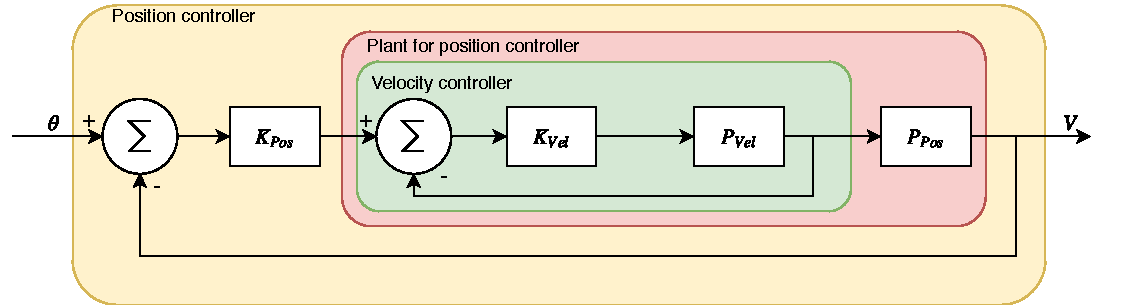
\includegraphics[width = 0.7 \textwidth]{Sections/System_Design/Images/cascade_controller.pdf}
    \caption{Block diagram of a cascaded controller. $K_{Pos}$ being the position controller, $K_{Vel}$ being the velocity controller, $P_{Vel}$ returns the velocity of the plant and $P_{Pos}$ returns the position of the plant.}
    \label{fig:cascaded_design}
\end{figure}
Figure \ref{fig:cascaded_design} shows the principles of the cascaded controller design. Designing the inner controller, i.e. the velocity controller has been described above. From the figure it can be seen that when designing the outer position controller, the inner controller has to be regarded as part of the plant. From figure \ref{fig:cascaded_design} the transfer function in equation \ref{eq:tf_cascaded_design} can be derived.
\begin{equation} \label{eq:tf_cascaded_design}
    \frac{\theta}{V}=\frac{K_{pos}\cdot\frac{K_{vel}\cdot P_{vel}}{1+K_{vel}\cdot P_{vel}}\cdot P_{pos}}{1+ K_{pos}\cdot\frac{K_{vel}\cdot P_{vel}}{1+K_{vel}\cdot P_{vel}}\cdot P_{pos}}
\end{equation}
Since it has been decided to focus on only designing velocity controllers for the tilt motor, it only makes sense to also focus the cascaded design on the tilt motor.
When considering the plant as the combination of the closed loop velocity control system and an integrator to transfer from velocity to position, the design approach is going to be the same as have been used throughout most of this section. 
Figure \ref{fig:RL_cascade} shows that as expected, the poles and zeros accruing to the closed loop velocity control systems, appear as open loop poles and zeros in the Root Locus plot of the position control system. To design the PID position controllers, very similar zero placements methods  are used. In the case of the model based velocity controller, zeros are placed at $s = 6.1$ and $s = 1.2$ while for the Ziegler-Nichols based controller zeros are placed at $s = 6.2$ and $s = 1$. Even though the zeros accruing to the PID controllers are placed almost identically, the Root Loci are quite different due to the different poles and zeros accruing to the velocity controllers. From the closed loop pole locations, it is expected that the response from the control system based on the Ziegler-Nichols tuning will have a faster response, but also quite a bit more overshoot. From the bode plots in figure \ref{fig:cascade_bode} it can be seen that the sampling frequency of \SI{1000}{\hertz} is still easily sufficient. From the phase and gain margins shown in figure \ref{fig:cascade_stability} it can be seen that the Ziegler-Nichols based design has a slightly smaller phase margin at \SI{75.7}{\degree} to the \SI{118}{\degree} of the model based design.
% If both the pole placement and Ziegler-Nichols approaches are examined, maybe they should be presented in the same plots.

\begin{figure}[h]
\begin{subfigure}{0.48\textwidth}
    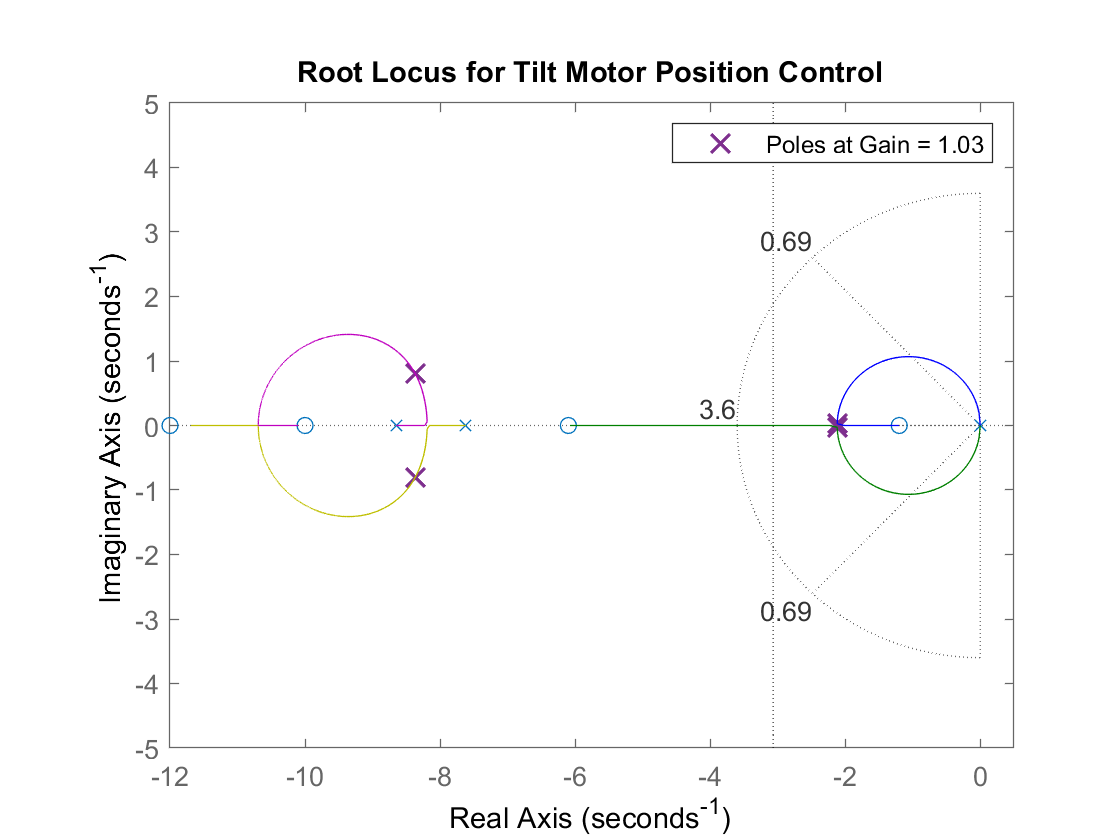
\includegraphics[width = 0.97\textwidth]{Sections/System_Design/Images/RL_cascadePP.png}
    \caption{Controller design based on model.}
    \label{fig:RL_cascade_PP}
\end{subfigure}\quad
\begin{subfigure}{0.48\textwidth}
    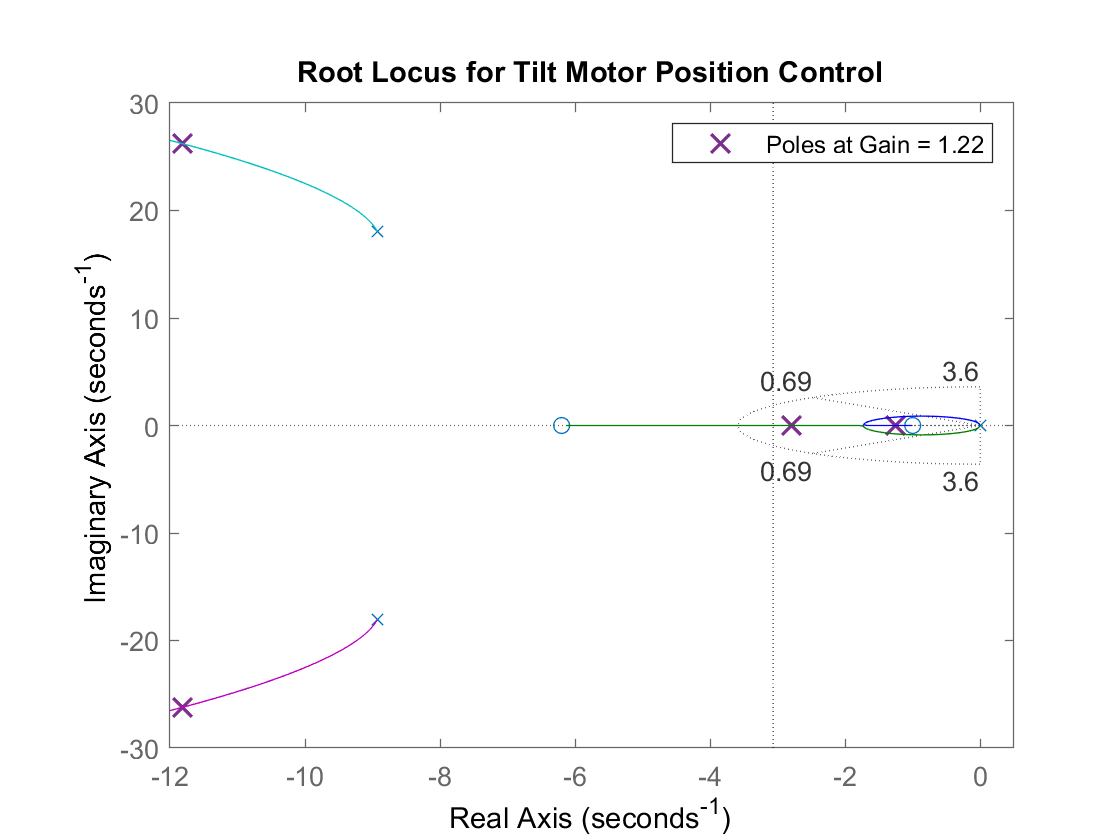
\includegraphics[width = 0.97\textwidth]{Sections/System_Design/Images/RL_cascadeNZ.png}
    \caption{Maybe add the bode plot the ziegler nichols here.}
    \label{fig:RL_cascade_NZ}
\end{subfigure}
\caption{Bode plots of the closed loop system with velocity controllers designed using the model and using the Ziegler-Nichols method.}
\label{fig:RL_cascade}
\end{figure}

Looking at the step responses for the two designs, shown in figure \ref{fig:cascade_step}, it can be seen that, ideally, both methods perform quite well in regards to the specifications in table \ref{tab:performanceSpec}, although the settling time requirement cannot quite be met. The Ziegler-Nichols based design gives slightly less overshoot, but does give a strange and unwanted transient response. This is only the case when saturation is not considered. In the case when saturation is considered, the Ziegler-Nichols based design performs better in terms of overshoot, while both give a settling time which does not quite comply with the specifications.

\begin{figure}[h]
\begin{subfigure}{0.48\textwidth}
    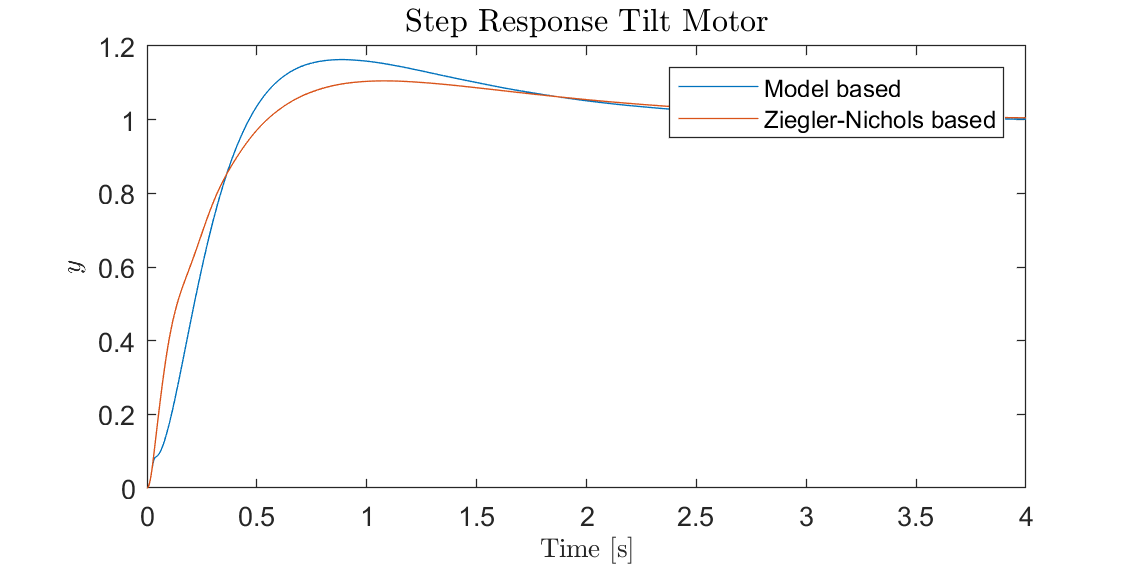
\includegraphics[width = 0.97\textwidth]{Sections/System_Design/Images/cascade_step_y_sat.png}
    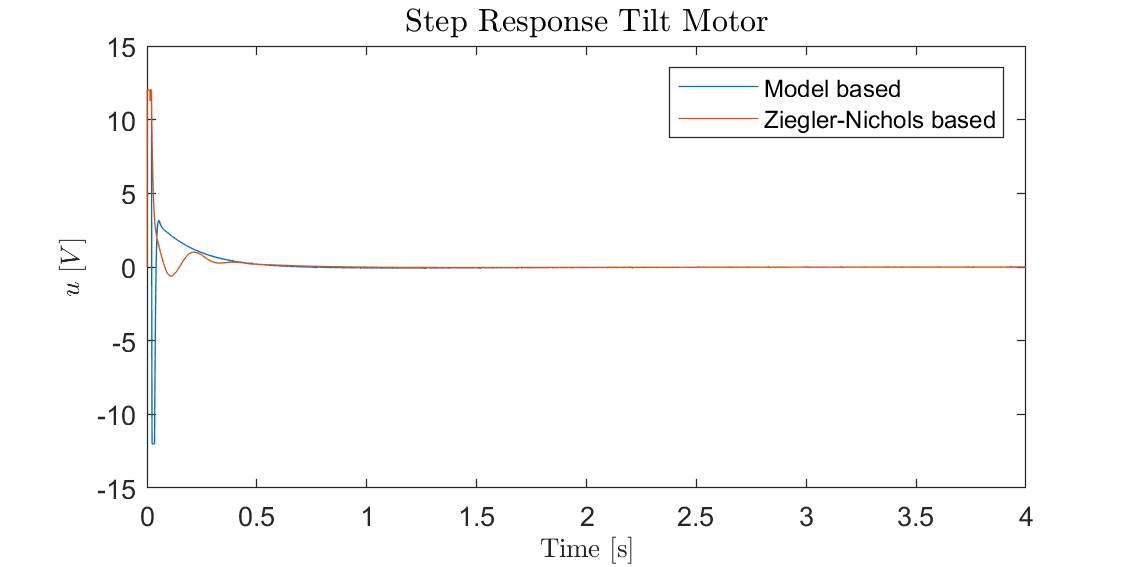
\includegraphics[width = 0.97\textwidth]{Sections/System_Design/Images/cascade_step_u_sat.png}
    \caption{Systems with saturation included.}
    \label{fig:RL_cascade_PP}
\end{subfigure}\quad
\begin{subfigure}{0.48\textwidth}
    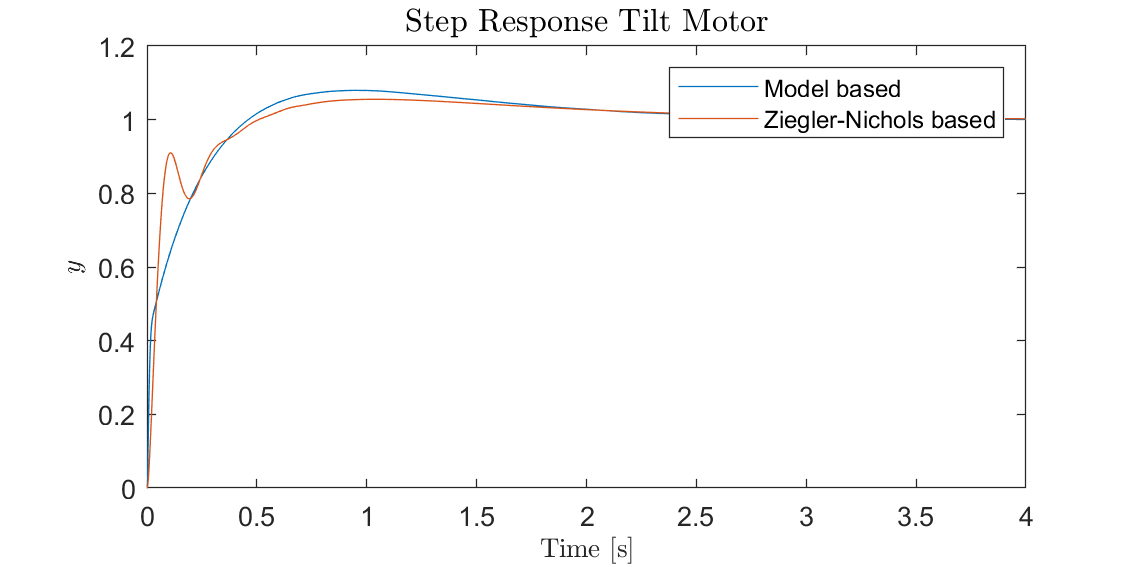
\includegraphics[width = 0.97\textwidth]{Sections/System_Design/Images/cascade_step_y_NoSat.png}
    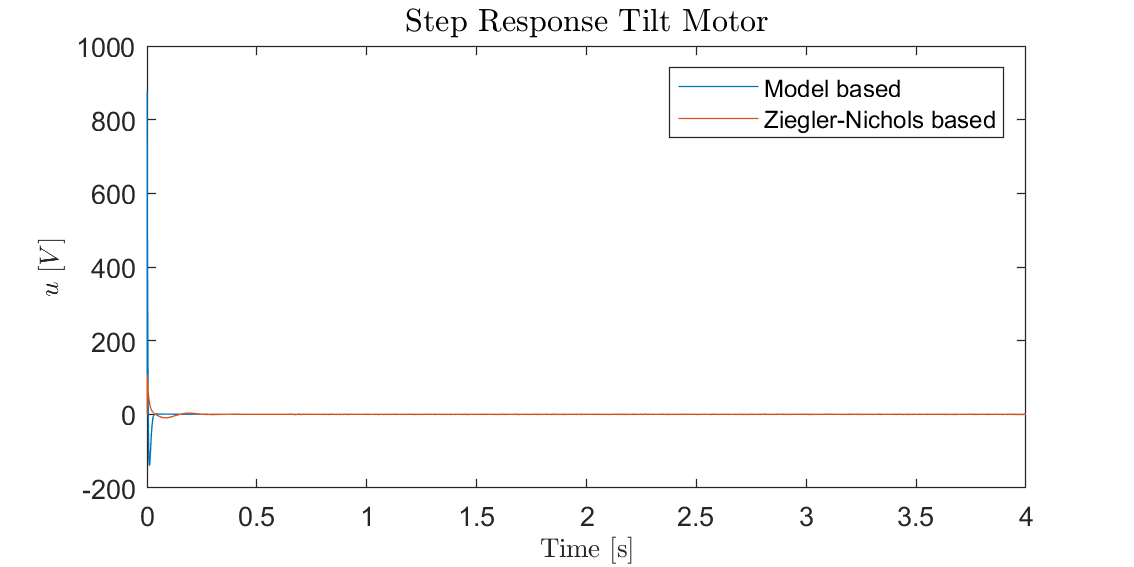
\includegraphics[width = 0.97\textwidth]{Sections/System_Design/Images/cascade_step_u_NoSat.png}
    \caption{Systems without saturation.}
    \label{fig:RL_cascade_NZ}
\end{subfigure}
\caption{Bode plots of the closed loop system with velocity controllers designed using the model and using the Ziegler-Nichols method.}
\label{fig:RL_cascade}
\end{figure}

% Present the root locus, maybe the bode plot, and the stability margins.
%present the step responses and discuss in relation to specifications
% If deemed relevant, the step response without saturation can be included in order to argue why it is normally not ideal to have overshoot on the velocity controller.



\subsection{Conclusion}

\end{document}